% vim: set tw=78 sts=2 sw=2 ts=8 aw et ai:
\documentclass[12pt]{article}

\usepackage[paper=a4paper, top=2cm, bottom=3cm, left=2.5cm, right=2.5cm]{geometry}

\usepackage{ucs}
\usepackage[utf8x]{inputenc}
\usepackage[english]{babel}
%\usepackage{hyperref}	  % use \url{http://$URL} or \href{http://$URL}{Name}
\usepackage{underscore}	  % underscores need not be escaped
\usepackage{subfigure}
\usepackage{verbatim}
\usepackage{float}
\usepackage{booktabs}     % professional tables

% Support for including graphics
\usepackage{graphicx}
\DeclareGraphicsExtensions{.pdf,.png,.jpg}

\title{VMchecker optimisation: algorithm for increasing speed of automatic
homework evaluation}

\author{Alexandru Juncu\\
Automatic Control and Computers Faculty\\
University POLITEHNICA of Bucharest\\
Splaiul Independenței nr. 313, Bucharest, Romania \\
\emph{alexandru.juncu@cs.pub.ro}}

\date{February 3rd, 2012}

\begin{document}

\maketitle

\begin{abstract}
% vim: set tw=78 sts=2 sw=2 ts=8 aw et ai:
The use of an automated testing system for homeworks or for contest
submissions is is commonly used in the academic world, specially in
computer science related fields. Such systems offer an efficient way of
collecting and storing homeworks and a quick, impartial, deterministic
and transparent way of grading them. An automated testing speeds up
considerably the grading time as compared to manual grading.

A secure implementation of a testing systems need some sort of containment
of the environment in which each test is ran. Different types of
virtualisation technologies can be used, from chroot jails to full
virtualisation, depending on the requirements of the tests.

An example of an automated homework testing system is a project called
\emph{VMchecker}. This open source tool is made up of several components,
among which a virtualisation infrastructure based on VMware Workstation.
VMchecker has been successfully deployed in academic environments and is
currently serving over 500 students each semester.

The following paper is focused around optimising VMchecker in order to
better prioritise homework submissions to achieve faster grading times and
scaling the infrastructure to support parallel homework evaluations.

In order to do this, statistics about the current implementation of
VMchecker has been gathered Following the analysis of the data, a new
algorithm is being proposed for implementation.

\end{abstract}
\pagebreak
\section{Introduction}
\label{sec:introduction}
% vim: set tw=78 sts=2 sw=2 ts=8 aw et ai:

VMchecker is an open sources project started by a group of teachers and
students from the Computer Science Department at the Politehnica University
of Bucharest. The goal was to automate testing of homework from the
Operating Systems and Compilers courses. Since then, it was been adopted by
several other courses, that had assessments ranging from high level
programming, to network simulations to kernel programming.

The architecture of VMchecker is very modular and uses several
technologies. The infrastructure is organized in three components:
\begin{itemize}
\item vmchecker-ui
\item vmchecker-storer
\item vmchecker-tester
\end{itemize}

The \emph{User Interface} is a web interfaces based on Google Web Toolkit,
a framework with a Java backend and a JavaScript frontend. The UI is used
by students to upload theit assessments, view the results of the automated
tests and view their final grade and feedback.

Assessments uploaded via the web UI, are stored in the repository, on the
\emph{Storer}. Each homework is archived in a Git repository. A student can
submit several revisions of the same assessment, each is tested, but only
the last one (current one) is displayed in the UI. The Storer manages a
queue of assessments that will be send out for checking. This component is
a collection of scripts written in Python or Bash and require 3rd party
modules like PyVix, an API for managing VMware virtual machines. Also on
the Storer, the tests for each homework are stored.

The submitted assessments from the queue on the Storer are passed to the
\emph{Tester}. The Tester has one or more virtual machines (VMware in the
current implementation) that can be started. After a fresh machine is
started, the generic homework tests are uploaded to the virtual machine,
then the submitted assessment. Both the tests and the submitted assessment
is compiled and the test is ran. The output of the tests is saved, along
with other system logs (like kernel logs in dmesg). The results are passed
back to the Stored, from where the UI can hand the results to the students.





\pagebreak
\section{Statistics analysis}
\label{sec:statistics}
% vim: set tw=78 sts=2 sw=2 ts=8 aw et ai:

The current implementation, although fully functional for the desired task,
has some inefficient resource usage and has been know to have periods when
performed below expectations.

In order to determine how to enhance VMchecker's performance, real life
statistics about how current VMchecker implementation performs. Taking data
from UPB Computer Science Department courses during an academic year and
analysing the number of submissions, the submission time, the duration of
the evaluation, we can determine the possible bottlenecks of the system and
find the places where improvements can be made.

Logs from submissions from several courses have been taken under
consideration. These courses vary from basic programming, operating systems programming or
administration, network administration to algorithms. Each has certain
constraints for containment test time and storage. Some run simple tests
that take a short time, others run simple tests but take more time, some
run tests that need root access on the machine, some need an input of a
single source file, others need the input of an entire virtual machine of
several gigabytes.

All submissions are treated almost the same (the virtual machine possibly
being different) with a First Come, First Served policy. If the tester can
run a single test at any one time, because a single virtual machine can be
started on the tester, bottlenecks are formed.

The pattern of the submissions isn't a constant line. There are moments
(ranging from minutes to days) where the checker isn't used and others
where several submissions are made almost at the same time.

Using data from two courses that take place in the same semester, each with
10 homework assignments, the patterns can be simply analysed. During the
course of a semester (14 weeks) about 13300 were made, out of which about
12400 were valid and actually tested. The times of the submissions and the
duration until results came in for that submissions where taking into
account measure the load of the infrastructure.

Figure \ref{fig:sub} shows the evolution of the number of submissions over
the semester. It is clearly visible the fact that the number of submissions
increases as headline for assignments come near. If two deadlines for
different courses overlap within a couple of days, the number peaks.

The relationship between the number of submissions and the average time to
get the results is shown by figure \ref{fig:sub}. Because of the first come
first serve algorithm and the fact that there is only one tester for all
the submissions means that if the number of submissions increases
considerably. If the first homework in the queue takes a certain time, the
next one will take twice as long before the results for it are returned.

\begin{figure}[H]
\begin{center}
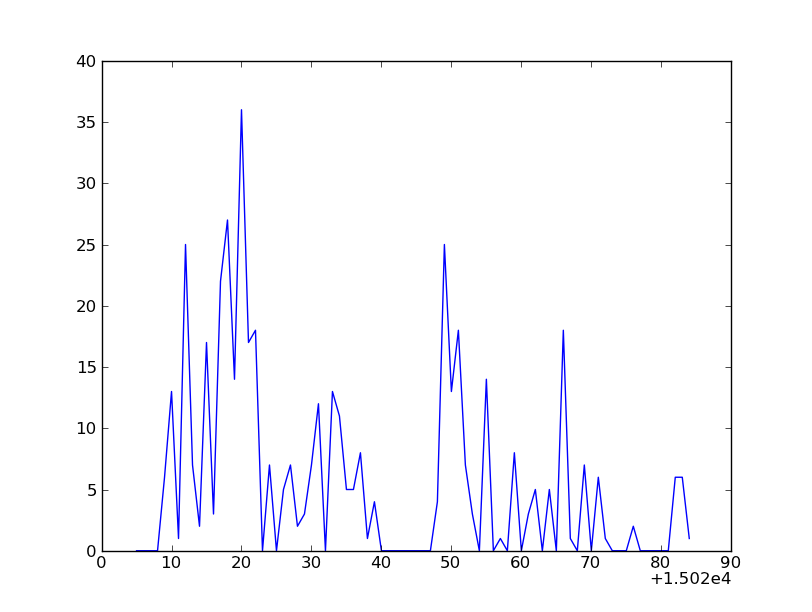
\includegraphics[height=0.4\textheight]{src/so}
\caption{Average number of submissions}
\label{fig:sub}
\end{center}
\end{figure}

\begin{figure}[H]
\begin{center}
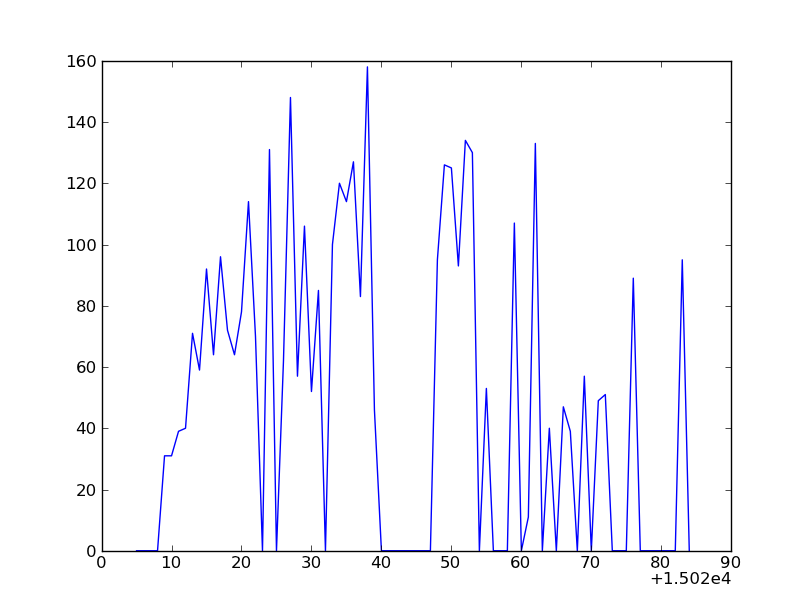
\includegraphics[height=0.4\textheight]{src/sotime}
\caption{Average time for testing}
\label{fig:time}
\end{center}
\end{figure}



\pagebreak
\section{Proposed Algorithm}
\label{sec:implementation}
% vim: set tw=78 sts=2 sw=2 ts=8 aw et ai:

The main bottleneck of the infrastructure is the Tester. The current
implementation of the Tester makes it possible for only one  VMware virtual
machine to be used at one time. This means that all submissions to be
tested need to wait in the same queue. Along with the First Come First
Serve policy, means that submissions at the back of the queue get processed
very slow.

The problem is similar to the one that network traffic faces. Internet
packets are different, some are big, some are small, some are processed
fast, some are processed slow. The default way that packets are routed is
on a First Come First Serve bases, which means that some packets get
treated worse than others. Without a Quality of Services implemented,
theres is no prediction of the treatment of important or unimportant
packets.

From data analysed, current instance of VMchecker has three types of
homework tests:
\begin{itemize}
\item simple tests that run only in userspace an require basic containment
of the test process
\item system or kernel level tests that require root access to the entire
virtual machine
\item full system tests that need the entire virtual machine to be taken as
input
\end{itemize}

The first step of optimising VMchecker is to mark these types of
assessments by the above categories. This means that the Tester will know
what is the estimated time of the testing and can be able to choose smaller
tests in front of bigger tests. If two simple tests that take tens of
seconds are submitted after a test that needs the entire virtual machine to
be copied, all of these will take a matter of minutes in average to get the
result. But if a QoS is implemented, the Tester can choose to run the
smaller tests first, even though the larger test was submitted first.

But as long as the tester can only run a single virtual machine, the queue
can still become long enough to provide bad result times. The obvious
solution is to run multiple virtual machines at the same time so that
several tests can be run simultaneously. But this require adequate hardware
resources.

Running more than one virtual machine on the Tester offers another
optimisation: provisioning machines. In the current implementation every
time a submission is made, the tester start the correct virtual machine for
that test. This takes time because the machine needs to be started or
resumed from a snapshot on the spot. Provisioning machines means that fresh
virtual machines are already started and ready to receive tests to be ran.
In the best case scenario, anytime a test needs to run, a machine is up and
running and is instantly ready to run the test. The machine is cleanup
(closed) after the test is done, but this won't affect the next test,
because that next test will run on another provisioned machine.

But the idea of provisioning brings another question: how many machines to
keep running and of what type? Keeping too many machines running that
aren't needed means that if only one is (or a few are) used, that (or
those) will perform bad because they need to share resources with the other
that are idle.

The proposed algorithm is based on all the optimisations mentioned above.
First of all, the types of virtual machines should vary. Simple tests can
be run on OpenVZ or LXC, rather than VMware full virtualization. The full
system tests could be run on other full virtualization or
paravirtualization like VirtualBox or Xen. Depending on the tests, the
appropriate machine should be used, because an OpenVZ machine is easier to
start and clean compared to a VMware machine, and if a test doesn't need
more than userspace access, resources shouldn't be wasted on it.

Machines should be already started before tests are submitted, meaning that
multiple machines need to be started at the same time. What machines should
be provisioned need to be chosen using an heuristic that takes under
consideration the deadlines of assignments and the live requests made by
the users. If in one day, the number of VMware machines are higher than
usual, OpenVZ machines could be stopped to reallocate resources to the
needed ones.


\section{Conclusion and Further Work}
\label{sec:conclusion}
% vim: set tw=78 sts=2 sw=2 ts=8 aw et ai:

The VMchecker is a very usefull tool for both students an teachers and is a
good framework to build uppon. Continuing its development to provide better
services to its users is both possible and could bring semnificant results
with rather small tweeks.

The next step is the implement the proposed improvements to VMchecker in
the open source project. Simulations of the new algorithm based on the
existing data of submissions could provided the expected results of the
implementation, but the real results can only be observed after
implementing the optimizations and monitoring the performance of the new
system.



\bibliographystyle{abbrv}
\bibliography{my-report}

\end{document}
